\documentclass[tikz,border=3pt]{standalone}
\usepackage[T1]{fontenc}
\usepackage{lmodern,pgfplots}
\pgfplotsset{compat=1.18}
\definecolor{gapblue}{HTML}{4477AA}
\definecolor{densered}{HTML}{EE7733}
\definecolor{directgreen}{HTML}{228833}
\definecolor{inkgray}{HTML}{343A40}
\definecolor{gridgray}{HTML}{DEE3E8}
\definecolor{pendinggray}{HTML}{AAB4BE}
\newcommand{\AllianceBadge}{\tikz[baseline=-.4ex,x=.65ex,y=.65ex]{\path[fill=gapblue] (-.7,.9)--(.7,.9)--(.7,-.2)--(0,-.9)--(-.7,-.2)--cycle;}}
\newcommand{\HordeBadge}{\tikz[baseline=-.4ex,x=.65ex,y=.65ex]{\path[fill=densered] (0,1)--(.75,0)--(.45,-.8)--(0,-.45)--(-.45,-.8)--(-.75,0)--cycle;}}
\begin{document}

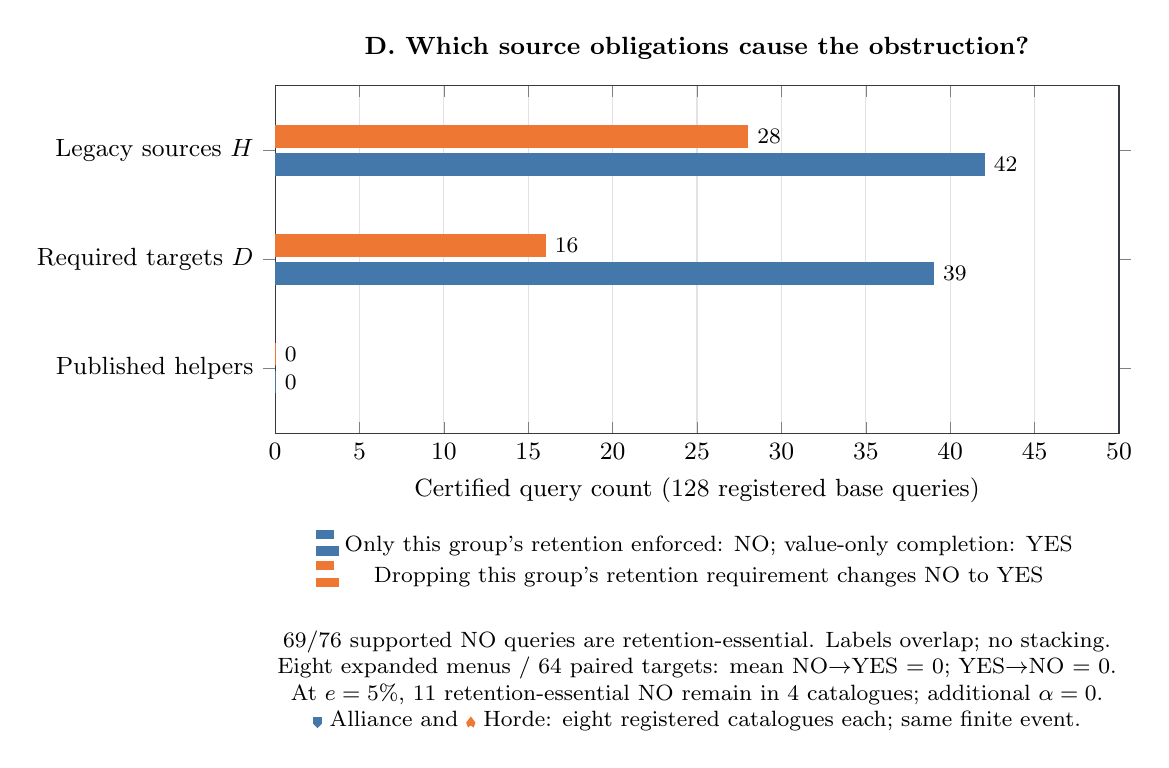
\begin{tikzpicture}
\begin{axis}[width=12.3cm,height=6cm,font=\small,xbar,bar width=8pt,xmin=0,xmax=50,
ytick={0,1,2},yticklabels={Published helpers,Required targets $D$,Legacy sources $H$},
xlabel={Certified query count (128 registered base queries)},
title={D. Which source obligations cause the obstruction?},title style={font=\small\bfseries},
ymin=-.6,ymax=2.6,xmajorgrids,grid style={gridgray},axis line style={inkgray},
legend style={at={(.5,-.26)},anchor=north,draw=none,font=\footnotesize,legend columns=1},
nodes near coords,point meta=x,every node near coord/.append style={font=\footnotesize},clip=false]
\addplot[fill=gapblue,draw=gapblue] coordinates {(42,2) (39,1) (0,0)};
\addlegendentry{Only this group's retention enforced: NO; value-only completion: YES}
\addplot[fill=densered,draw=densered] coordinates {(28,2) (16,1) (0,0)};
\addlegendentry{Dropping this group's retention requirement changes NO to YES}
\node[anchor=north,align=center,font=\footnotesize] at (axis description cs:.5,-.54) {69/76 supported NO queries are retention-essential. Labels overlap; no stacking.\\
Eight expanded menus / 64 paired targets: mean NO$\to$YES = 0; YES$\to$NO = 0.\\
At $e=5\%$, 11 retention-essential NO remain in 4 catalogues; additional $\alpha=0$.\\
\AllianceBadge\ Alliance and \HordeBadge\ Horde: eight registered catalogues each; same finite event.};
\end{axis}
\end{tikzpicture}
\end{document}
